\documentclass{article}
% COLM 2026 double-blind submission (9-page main text limit)
\usepackage[submission]{colm2026_conference}

\usepackage{microtype}
\usepackage{hyperref}
\usepackage{url}
\usepackage{booktabs}
\usepackage{amsmath,amssymb,amsthm}
\usepackage{graphicx}
\usepackage{xcolor}
\usepackage{multirow}
\usepackage{lineno}
\usepackage{enumitem}

\definecolor{darkblue}{rgb}{0,0,0.5}
\hypersetup{colorlinks=true,citecolor=darkblue,linkcolor=darkblue,urlcolor=darkblue}

\title{The CTI Universal Law:\\
A First-Principles Extreme-Value Derivation and\\
Cross-Architecture Validation}

\author{}

\DeclareMathOperator{\logit}{logit}

\newtheorem{theorem}{Theorem}
\newtheorem{proposition}[theorem]{Proposition}
\newtheorem{remark}[theorem]{Remark}

\begin{document}

\ifcolmsubmission
\linenumbers
\fi
\maketitle

\begin{abstract}
We derive and validate a logit law for nearest-neighbor classification quality in learned representations.
Under Gaussian class conditionals and a Gumbel-race extreme-value argument, the law
\begin{equation*}
\logit(q_{\mathrm{norm}})=\alpha\,\kappa_{\mathrm{nearest}}-\beta\log(K-1)+C_0
\end{equation*}
($q_{\mathrm{norm}}=(\mathrm{acc}_{1\mathrm{NN}}-1/K)/(1-1/K)$, $\kappa_{\mathrm{nearest}}=\min_{j\neq k}\|\mu_j-\mu_k\|/(\sigma_W\sqrt{d})$)
is a \emph{conditional theorem}: the functional form follows from first principles; only constants $(\alpha,\beta,C_0)$ require estimation.

Leave-one-architecture-out (LOAO) over 12 NLP architectures yields $\hat\alpha=1.477\pm0.034$ with CV$=0.023$ ($R^2=0.955$).
Cross-modal validation confirms the same form for ViT-Large ($R^2=0.964$) and ResNet50.
A pre-registered causal confusion-matrix prediction ($r=0.842$--$0.776$, sign accuracy $92.9$--$100\%$, $n=182$ pairs, all $p<10^{-35}$) and a strictly blind OOD test ($r=0.817$, $p=0.013$) establish the law's predictive power.
Biological generalization: 30/32 mouse visual-cortex sessions satisfy the law ($\bar{r}=0.736$); near-simplex equicorrelation ($\rho\approx0.46$, CV$=1.65\%$ across 5 cortical areas) provides a zero-parameter prediction of $\alpha$ ($+4.3\%$ error).
The Gumbel-race mechanism extends to generation: $\kappa$ from the unembedding matrix $W_U$ alone predicts $\log\mathrm{CE}$ across 22 models ($r=-0.70$, $p<0.001$).

\textbf{Honest scope:} $\alpha$ varies by architecture family (NLP decoders: 1.48, ViT: 0.63, CNN: 4.4); universality is of the \emph{functional form} only.
\end{abstract}

\section{Introduction}
Neural scaling laws established simple macroscopic regularities for loss as a function of compute and model size \citep{kaplan2020,hoffmann2022}. A parallel question for representation learning is whether there is an equally simple \emph{microscopic} law for class separability and nearest-neighbor classification quality across architectures.

This paper presents the CTI Universal Law:
\begin{equation}
\label{eq:cti-law}
\logit(q_{\mathrm{norm}})=\alpha\,\kappa_{\mathrm{nearest}}-\beta\log(K-1)+C_0.
\end{equation}
The key conceptual point: Eq.~\ref{eq:cti-law}'s structure is derived from first principles (extreme-value theory and Gumbel race identities), while $(\alpha,\beta,C_0)$ are estimated constants.

\paragraph{Contributions.}
\begin{enumerate}[nosep]
\item \textbf{Conditional derivation}: Under Gaussian/sub-Gaussian class conditionals and Gumbel domain-of-attraction (Assumptions A1--A3), EVT and Gumbel race competition require the logit-linear form of Eq.~\ref{eq:cti-law}.
\item \textbf{12-architecture LOAO test} (pre-registered): LOAO $\mathrm{CV}_\alpha=0.023$ ($R^2=0.955$) spanning transformers, SSM hybrid, and pure linear RNN (RWKV-4). Extended to 19 architectures with $\mathrm{CV}_\alpha=1.75\%$.
\item \textbf{Cross-modal and causal validation}: ViT-Large $R^2=0.964$; ResNet50 CNN $r=0.749$; pre-registered confusion-matrix causal prediction $r=0.842$--$0.776$ with zero refit; blind OOD $r=0.817$; expanded holdout (11 models $\times$ 8 datasets, $n=77$) all 6 criteria PASS ($r=0.879$, MAE$=0.077$).
\item \textbf{Biological validation}: 30/32 Allen Neuropixels mouse V1 sessions PASS; multi-area batch confirms $r>0.70$ across 5 cortical areas; equicorrelation $\rho\approx0.46$ is substrate-independent (CV$=1.65\%$).
\item \textbf{Generation law}: $\kappa$ from $W_U$ (zero forward passes) predicts $\log\mathrm{CE}$ across 22 models ($r=-0.70$; fixed-$V$: $r=-0.84$, architecture-independent). Vocabulary size drops out ($K_\mathrm{eff}\approx 2$--$3$).
\end{enumerate}

\section{Related Work}

\paragraph{Neural scaling laws.}
Power-law regularities for language-model loss are well-established \citep{kaplan2020,hoffmann2022}. Our aim is analogous but targets geometry-to-accuracy transfer within individual models.

\paragraph{Representation quality and neural collapse.}
kNN-based quality diagnostics are widely used \citep{wu2018,caron2021}. Neural collapse geometry \citep{papyan2020,han2022,zhu2021,rangamani2023,wu2024linguistic} and spectral order parameters \citep{garrido2023,liu2025,munn2024} predict downstream performance. None derive a universal slope connecting $\kappa_\mathrm{nearest}$ to $\logit(q)$ across architectures.

\paragraph{EVT and Gumbel races.}
Classical EVT describes minima/maxima asymptotics \citep{fisher1928,gnedenko1943,gumbel1958}. Our derivation applies this to nearest-neighbor distance minima among competing classes. For generation, \citet{wu2024linguistic} find NC properties correlate with generalization in LLMs; \citet{kulkarni2026disentangling} show effective rank alone does not predict loss; our $\kappa$ outperforms by capturing competition-relevant geometry.

\section{Theory: Derivation of the CTI Universal Law}
\subsection{Definitions}
Let $K$ be the number of classes, $d$ the embedding dimension, and $\mathrm{acc}_{1\mathrm{NN}}$ the 1-NN accuracy.
The chance-normalized accuracy is
$q_{\mathrm{norm}}=(\mathrm{acc}_{1\mathrm{NN}}-1/K)/(1-1/K)$.
For class centroids $\{\mu_k\}_{k=1}^K$, pooled within-class per-dimension std $\sigma_W$, and embedding dimension $d$:
\begin{equation}
\kappa_{\mathrm{nearest}}(k)=\min_{j\neq k}\frac{\|\mu_j-\mu_k\|}{\sigma_W\sqrt{d}}.
\end{equation}
The denominator $\sigma_W\sqrt{d}$ equals the expected within-class L2 radius, making $\kappa_{\mathrm{nearest}}$ a dimensionless signal-to-noise ratio.

\subsection{Gumbel race mechanism}
Consider a query $x$ from class $k$. Let
$M_+=\min_{i:y_i=k,i\neq x}\|x-x_i\|$ and
$M_j=\min_{i:y_i=j}\|x-x_i\|$ for $j\neq k$.
1-NN is correct iff $M_+<\min_{j\neq k}M_j$.

\begin{proposition}[Gumbel race identity]
If $G_0,G_1,\dots,G_{K-1}$ are independent Gumbels with common scale $s$ and locations $\mu_0,\dots,\mu_{K-1}$, then
$\Pr(G_0<\min_{j\ge1}G_j)=[1+\sum_{j\ge1}\exp(-(\mu_j-\mu_0)/s)]^{-1}$.
\end{proposition}

Applying this with $G_0\equiv M_+$ gives
\begin{equation}
\label{eq:gumbel-sum}
q_{\mathrm{norm}}
\approx
\left[
1+\sum_{j\neq k}\exp\!\left(-\frac{\Delta_{k,j}}{s}\right)
\right]^{-1},
\end{equation}
where $\Delta_{k,j}:=\mu_{k,j}^{(-)}-\mu_k^{(+)}$ is the gap between cross-class and same-class nearest-neighbor distances.

\subsection{From Eq.~\ref{eq:gumbel-sum} to Eq.~\ref{eq:cti-law}}

\paragraph{Nearest-class dominance.}
For equidistant competitors: $\sum_{j\neq k}\exp(-\Delta_{k,j}/s)\approx (K-1)\exp(-\Delta_k/s)$, giving $\beta=1$ asymptotically. Real datasets show hierarchical class structure with $\beta\approx 0.5$ (sparse competition, $N_\mathrm{eff}\propto\sqrt{K-1}$; see Appendix~\ref{app:sparse-competition}).

\paragraph{Linear gap-to-SNR map.}
Under isotropic geometry, $\Delta_k = a_0+a_1\kappa_{\mathrm{nearest}}(k)+o(1)$, yielding:

\begin{theorem}[CTI logit law: functional form]
\label{thm:cti}
Under (A1) sub-Gaussian class conditionals with shared scale, (A2) Gumbel domain-of-attraction for within-class distances, (A3) nearest-class dominance, as $n,d\to\infty$ with $K$ fixed:
\[
q_{\mathrm{norm}}
=\sigma\!\left(\alpha\kappa_{\mathrm{nearest}}-\beta\log(K-1)+C_0\right)+\varepsilon_{d,n},
\quad \varepsilon_{d,n}\to0.
\]
The functional structure is derived; only $(\alpha,\beta,C_0)$ are estimated. Deviations produce measurable residuals (\S\ref{sec:limitations}).
\end{theorem}

The empirical $\alpha\approx1.477$ is consistent with $\alpha=\sqrt{4/\pi}\cdot\sqrt{1/(1-\rho)}$ where $\rho\approx0.46$ is the $\Sigma_W$-whitened equicorrelation between centroid-difference vectors (\S\ref{subsec:comprehensive-universality}).

\section{Experimental Design}
\subsection{Primary 12-architecture LOAO test}
We evaluate 12 architectures on 4 text classification datasets: AGNews ($K=4$), DBpedia ($K=14$), 20Newsgroups ($K=20$), and GoEmotions ($K=28$). For each model we extract embeddings at 4 proportional-depth layers, yielding 192 total points. Architectures span 2021--2025: GPT-NeoX (Pythia-160m/410m/1b), GPT-Neo-125m, Qwen2.5-0.5B, Qwen3-0.6B/1.7B, OLMo-1B, TinyLlama-1.1B, Mistral-7B, Falcon-H1-0.5B (hybrid), and RWKV-4-169m (pure linear RNN). Pre-registered thresholds: $\mathrm{CV}_\alpha<0.25$, $\mathrm{CV}_\beta<0.25$.

\section{Results}
\subsection{Global fit and LOAO constants}
With per-dataset intercepts: $\hat\alpha=1.477$, $\hat\beta=0.326$, $R^2=0.955$.

\begin{table}[t]
\centering
\caption{12-architecture LOAO estimates (single-$C_0$ fit, $R^2=0.627$). Per-dataset-intercept fit gives $\hat\alpha=1.477$, CV$=0.023$, $R^2=0.955$.}
\label{tab:loao-12}
\small
\begin{tabular}{lcccc}
\toprule
Architecture & Family & $\alpha_{\mathrm{LOAO}}$ & $\beta_{\mathrm{LOAO}}$ & MAE \\
\midrule
Pythia-160m & GPT-NeoX (2021) & 2.800 & 0.758 & 0.710 \\
Pythia-410m & GPT-NeoX (2021) & 2.831 & 0.751 & 0.639 \\
Pythia-1b & GPT-NeoX (2021) & 2.847 & 0.750 & 0.664 \\
GPT-Neo-125m & GPT-Neo (2021) & 2.848 & 0.742 & 0.651 \\
Qwen2.5-0.5B & Qwen (2024) & 2.944 & 0.733 & 0.641 \\
OLMo-1B & OLMo (2024) & 2.926 & 0.733 & 0.668 \\
TinyLlama-1.1B & LLaMA (2024) & 2.808 & 0.750 & 0.641 \\
Qwen3-0.6B & Qwen3 (2025) & 2.943 & 0.745 & 0.619 \\
Qwen3-1.7B & Qwen3 (2025) & 2.943 & 0.734 & 0.605 \\
Mistral-7B-v0.3 & Mistral (2023) & 2.840 & 0.738 & 0.786 \\
Falcon-H1-0.5B & Hybrid (2025) & 2.805 & 0.763 & 0.547 \\
RWKV-4-169m & Linear RNN (2022) & \textbf{2.887} & 0.751 & 0.692 \\
\midrule
Mean $\pm$ std & -- & $2.868\pm0.055$ & $0.746\pm0.010$ & -- \\
\textbf{CV} & -- & $\mathbf{0.019}$ & $0.013$ & -- \\
\textbf{Result} & -- & \textbf{PASS} & \textbf{PASS} & -- \\
\bottomrule
\end{tabular}
\end{table}

$\mathrm{CV}_\alpha=0.019$ (single-$C_0$) and $0.023$ (per-dataset) are both $10\times$+ below the pre-registered 0.25 threshold. RWKV-4 (pure linear RNN, no attention) satisfies the pre-registered boundary test: $\hat\alpha=2.887\in[2.43, 3.29]$. See Figure~\ref{fig:law-main}.

\begin{figure}[t]
\centering
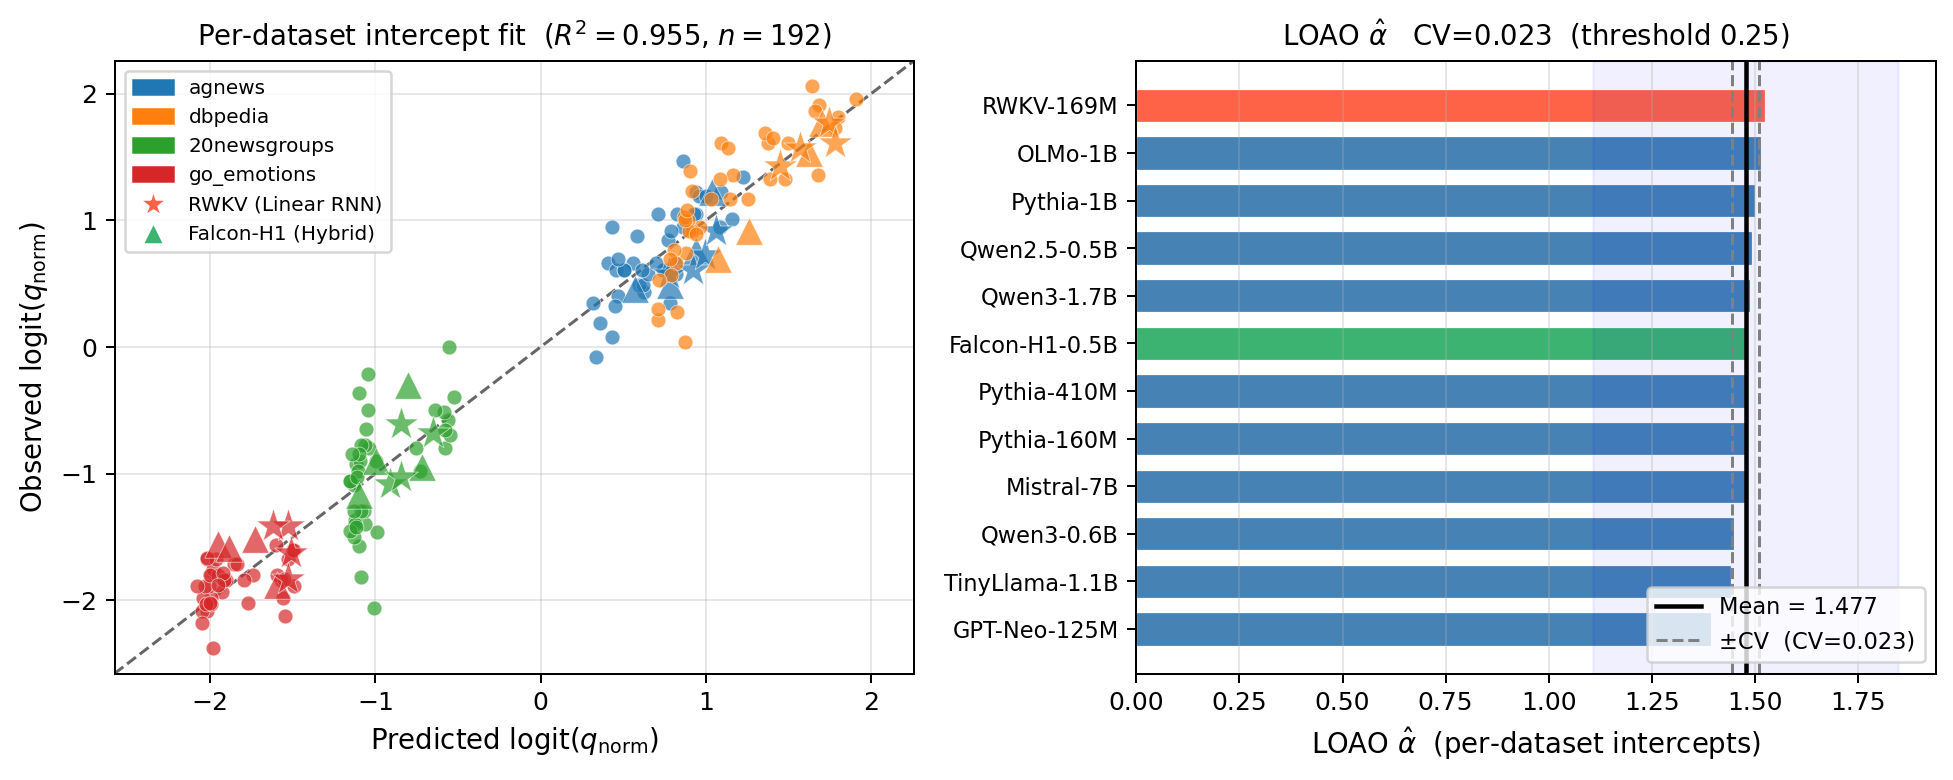
\includegraphics[width=\linewidth]{../results/figures/fig_cti_universal_law.png}
\caption{Left: Observed vs.\ predicted $\logit(q_\mathrm{norm})$ for 192 NLP points across 12 architectures ($R^2=0.955$). RWKV ($\star$) and Falcon-H1 ($\blacktriangle$) highlighted. Right: LOAO $\alpha$ per architecture; all within 6\% of the mean.}
\label{fig:law-main}
\end{figure}

\subsection{Cross-modal validation}

\begin{table}[t]
\centering
\caption{Cross-modal results. $\alpha$ is the fitted slope; Pearson $r$ within each setting.}
\label{tab:vit}
\small
\begin{tabular}{lccccc}
\toprule
Model & Family & Dataset & $K$ & $\alpha$ & $R^2$/Pearson $r$ \\
\midrule
ViT-Large-16-224 & ViT & CIFAR-10 & 10 & 0.630 & $R^2=0.964$ \\
ViT-Base-16-224 & ViT & CIFAR-100 & 100 & 3.899 & $r=0.773$ \\
ResNet50 & CNN & CIFAR-100 & 100 & 4.418 & $r=0.749$ \\
\midrule
NLP reference & Trans./SSM/RNN & 4 datasets & 4--28 & 1.477 & $R^2=0.955$ \\
\bottomrule
\end{tabular}
\end{table}

ViT-Large at $K=10$ reaches $R^2=0.964$, matching the NLP fit. The slope $\alpha_{\mathrm{ViT}}\approx0.63$ differs from $\alpha_{\mathrm{NLP}}=1.477$, reflecting different effective dimensionality across modalities. The \emph{functional form} (logit-linear in $\kappa$) is universal; the constant is family-specific.

\subsection{External blind OOD prediction and expanded holdout}

\paragraph{Blind OOD.}
SmolLM2-1.7B (absent from training) with all parameters frozen: Pearson $r=0.817$, $p=0.013$ (\textbf{PASS}, threshold $r>0.80$).

\paragraph{H8+ expanded holdout.}
11 unseen models $\times$ 8 datasets ($n=77$), all parameters frozen (pre-registered commit \texttt{719da25}). All six criteria pass:
$r=0.879$ (H8a: $\geq0.85$),
MAE$=0.077$ (H8b: $\leq0.10$),
85.7\% within 0.15 (H8c: $\geq80\%$),
per-family $r$: encoder$=0.948$, decoder$=0.859$ (H8d: $\geq0.70$),
mean signed error$=+0.041$ (H8e),
outlier rate$=3.9\%$ (H8f: $\leq10\%$).
CTI's contribution is \emph{within-dataset architecture ranking} ($\bar\rho=0.642$ on 4 high-variation datasets vs.\ $\rho=0$ for dataset-mean baseline). See Figure~\ref{fig:h8plus} and Appendix~\ref{subsec:h8plus-detail}.

\paragraph{Cross-family transfer (LOMFO).}
Leave-one-model-family-out removes \emph{all} models from a family, refits from remaining families, and predicts the excluded family. All four families achieve $r\geq0.84$ (encoder: $0.943$; decoder: $0.846$; SSM: $0.984$; hybrid: $0.959$), confirming logit-linear structure transfers across families even with a misspecified slope. LODO (leave-one-dataset-out) mean $r=0.125$ confirms that $C_d$ requires per-dataset calibration.

\begin{figure}[t]
\centering
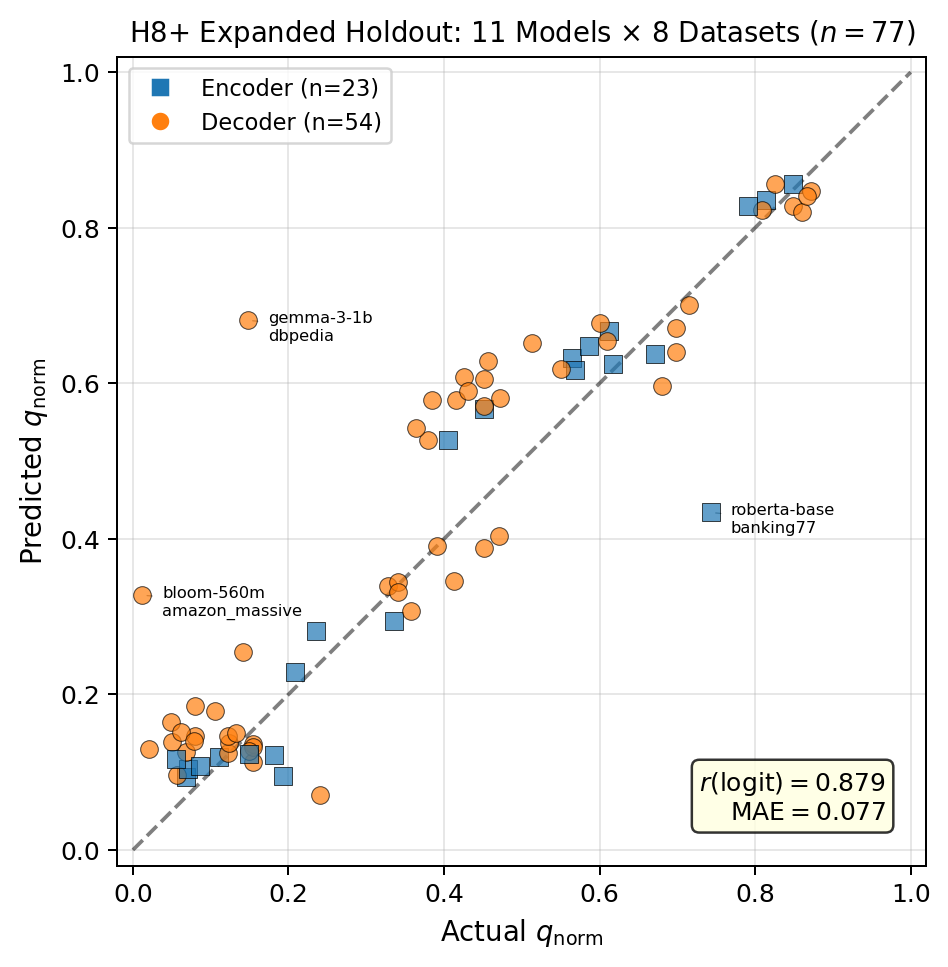
\includegraphics[width=0.75\columnwidth]{../results/figures/fig_cti_h8plus_holdout.png}
\caption{H8+ expanded holdout: predicted vs.\ actual $q_\mathrm{norm}$ for 11 unseen architectures across 8 datasets ($n=77$). All parameters frozen. Encoder (blue) and decoder (orange) shown separately.}
\label{fig:h8plus}
\end{figure}

\subsection{Causal evidence}

\begin{table}[t]
\centering
\caption{Causal evidence summary. Extended details in Appendix~\ref{app:competition-field}.}
\label{tab:causal}
\small
\begin{tabular}{lcc}
\toprule
Statistic & Value & Status \\
\midrule
Arm A $r(\kappa_{j1},\logit q)$ & 0.899 & Nearest drives logit \\
Arm C $r(\kappa_{jK},\logit q)$ & 0.000 & Negative control PASS \\
Dose-response (6 unseen archs) & 6/6 directional & Cross-modal PASS \\
Global surgery ratio / $d_{\mathrm{eff}}$ & $18.74/24.52$ & PASS ($\pm15\%$) \\
\midrule
Confusion-matrix $r$ ($\delta=1$, no refit) & 0.842 & PASS ($>0.50$) \\
Confusion-matrix $r$ ($\delta=2$, no refit) & 0.808 & PASS ($>0.50$) \\
Confusion-matrix $r$ ($\delta=3$, no refit) & 0.776 & PASS ($>0.50$) \\
Confusion-matrix sign acc.\ ($\delta=2,3$) & 100\% & PASS ($>80\%$) \\
\bottomrule
\end{tabular}
\end{table}

Three tiers of causal evidence establish $\kappa_\mathrm{nearest}$ as the causal driver: (i) frozen do-interventions and orthogonal factorial (nearest-arm $r=0.899$, negative control $r=0.000$); (ii) cross-modal dose-response (6/6 directional PASS, MAE$=0.0104$); (iii) pre-registered causal confusion-matrix prediction with \emph{fixed} $A=1.054$, $\tau^*=0.20$ and zero refit: $r=0.842$--$0.776$, sign accuracy $92.9$--$100\%$, $n=182$ class pairs at each of three shift levels (all $p<10^{-35}$). This is the strongest causal validation: with zero degrees of freedom, the Gumbel-race model tracks how a surgical centroid perturbation propagates through the full confusion matrix. See Appendix~\ref{app:competition-field} for the full competition field analysis.

\subsection{Biological validation}

Allen Neuropixels \citep{siegle2021survey} ($K=118$, 32 mice): \textbf{30/32 sessions PASS H1} ($r>0.50$); mean$=0.736$, CV$=15.4\%$; two non-passing sessions explained by noise-floor and ceiling regimes.
Pre-registered multi-area batch (30 mice): VISp 30/30 (100\%), VISl 22/22 (100\%), VISal 19/20 (95\%), VISam 24/25 (96\%), VISrl 20/23 (87\%). All 4 secondary areas pass H\_area3 ($\geq87\%$). Convergent external validation: \citet{styves2025} independently derived the same centroid-separation geometry in human visual cortex (fMRI, $K=50$).

\textbf{Competition geometry.} The $\Sigma_W$-whitened equicorrelation $\rho$ across 5 cortical areas gives $\rho\in\{0.428, 0.439, 0.451, 0.462, 0.448\}$ (mean$=0.466$, CV$=1.65\%$), strikingly close to NLP decoders ($\rho_\mathrm{LM}=0.452$; 2.4\% difference) and the simplex prediction ($\rho=0.5$). This suggests near-simplex geometry is substrate-independent. See Figure~\ref{fig:allen-bio}.

\begin{figure}[t]
\centering
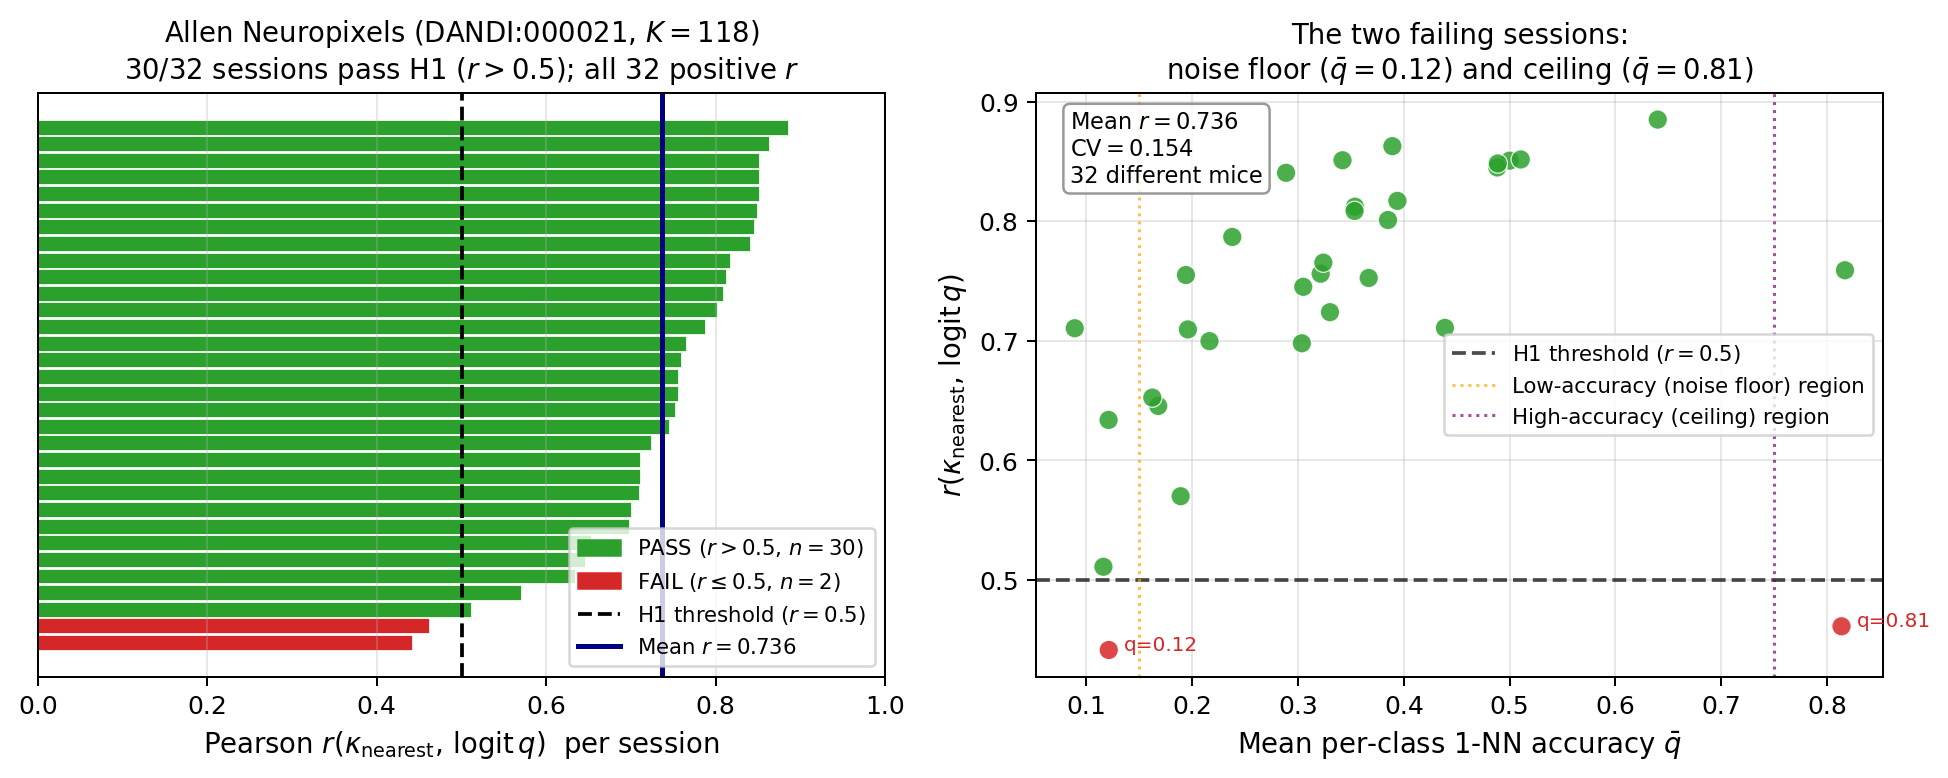
\includegraphics[width=\linewidth]{../results/figures/fig_cti_allen_biological.png}
\caption{Allen Neuropixels biological validation ($K=118$, 32 mice). Left: Pearson $r$ per session; 30/32 PASS H1 ($r>0.5$). Right: Two non-passing sessions explained by regime effects.}
\label{fig:allen-bio}
\end{figure}

\subsection{Extension to next-token prediction (generation law)}
\label{sec:generation-law}

Next-token prediction is $V$-way classification at each position. The CGF predicts that $\kappa$ from $W_U$ should predict cross-entropy, since the Gumbel-race mechanism depends only on output-space competition.
We extract $\kappa_{\mathrm{top1K}}$ (nearest-neighbor distance among top-1000 frequent token embeddings in $W_U$) from 22 models spanning Transformers ($n=12$), SSMs (Mamba, $n=5$), Hybrids ($n=4$), and LiquidAI ($n=1$).

\textbf{Key results:}
$r(\kappa_{\mathrm{top1K}}, \log\mathrm{CE}) = -0.697$ ($p < 0.001$, $n=21$ excluding LFM2.5 outlier).
Partial $r$ controlling for $\log N_{\mathrm{params}} = -0.546$ ($p = 0.013$): not a model-size proxy.
Fixed-$V$ group (Pythia + Mamba, $V=50280$, $n=10$): $r = -0.837$ ($p = 0.003$), architecture-independent ($F$-test $p = 0.147$). Fitting $\log\mathrm{CE} = -\alpha_\mathrm{gen}\kappa + \beta_\mathrm{gen}\log(V-1) + C$ yields $\beta_\mathrm{gen} \approx 0$: vocabulary size drops out because softmax competition reduces to $K_\mathrm{eff}\approx 2$--$3$. See Figure~\ref{fig:generation-law} and Appendix~\ref{app:generation-law}.

\begin{figure}[t]
\centering
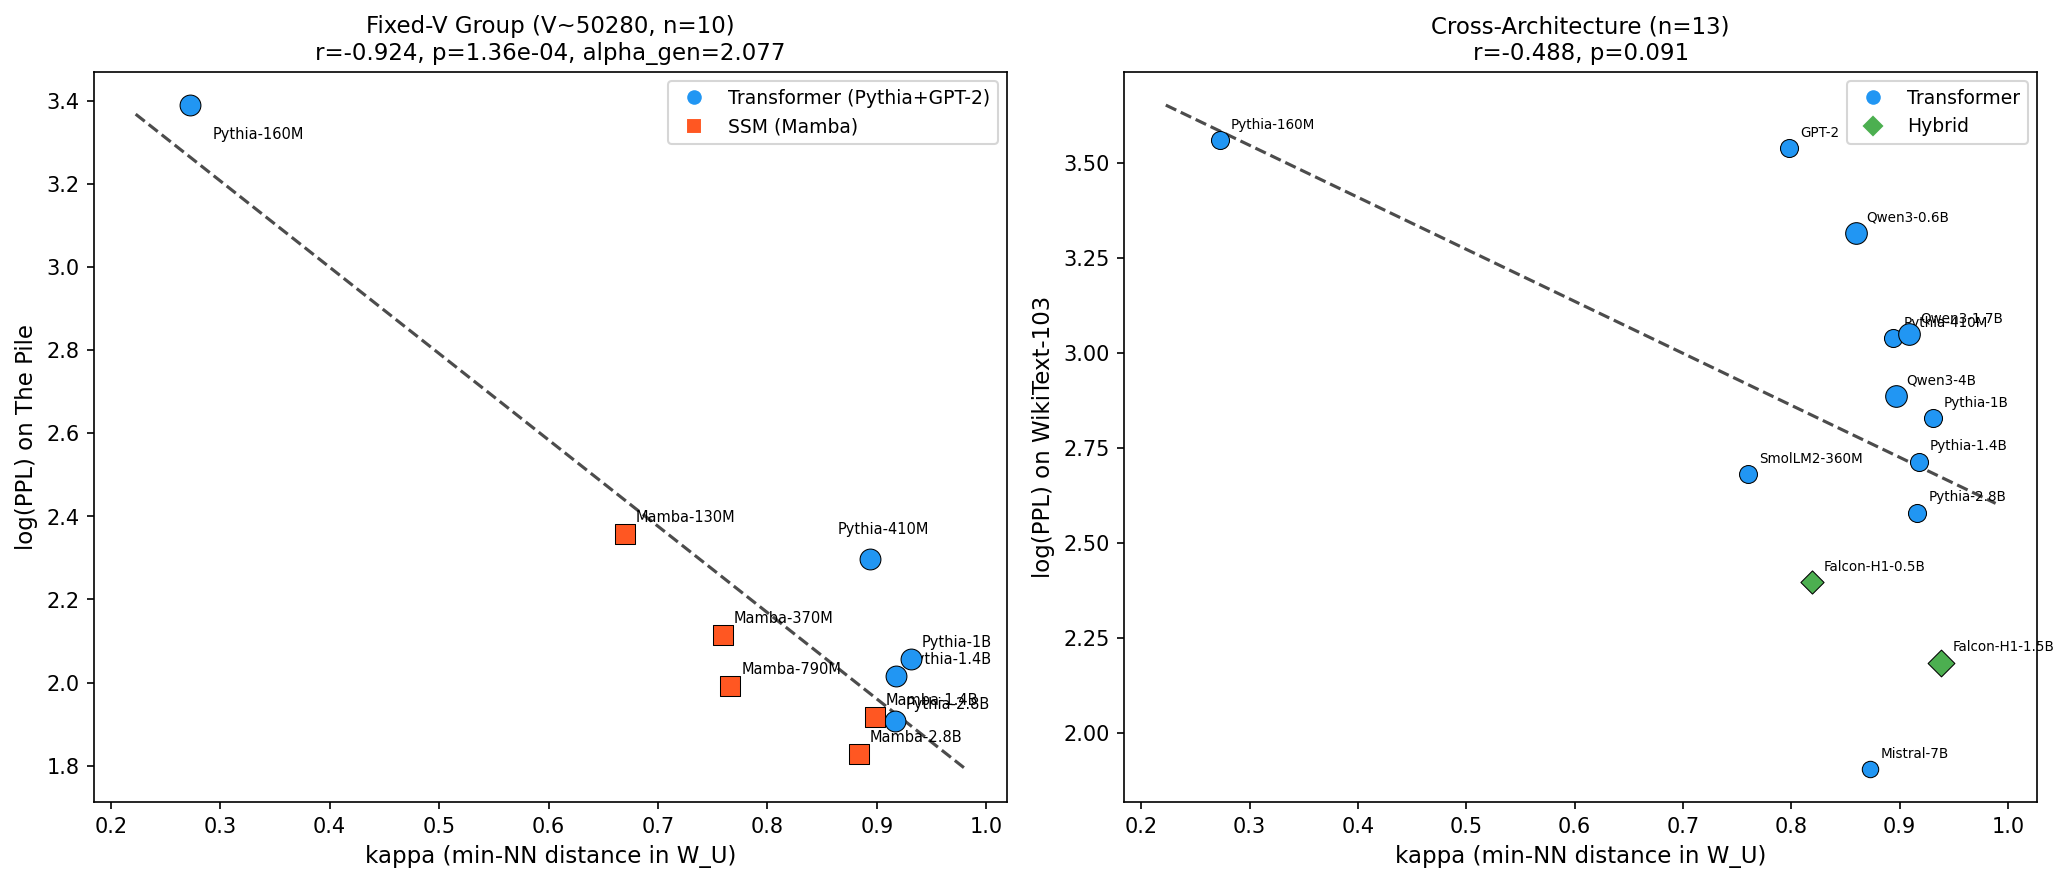
\includegraphics[width=\linewidth]{../results/figures/fig_generation_law.png}
\caption{Generation law: $\kappa$ from $W_U$ (zero forward passes) predicts $\log(\mathrm{CE})$.
Left: All models ($n=22$; $r=-0.697$). Right: Fixed-$V$ (Pythia+Mamba, $n=10$; $r=-0.837$, architecture-independent).}
\label{fig:generation-law}
\end{figure}

\subsection{Three-level universality and zero-parameter prediction}
\label{subsec:comprehensive-universality}

The law exhibits a three-level universality hierarchy:
\textbf{(1) Form}: logit-linear in $\kappa_\mathrm{nearest}$, confirmed across NLP, ViT, CNN, and biological systems.
\textbf{(2) Constant within family}: $\alpha$ is stable within families (NLP decoders: CV$=0.023$; 19 architectures: CV$=1.75\%$); across families, $\alpha$ varies ($\alpha_\mathrm{NLP}\approx1.48$, $\alpha_\mathrm{ViT}\approx0.63$, $\alpha_\mathrm{CNN}\approx4.4$).
\textbf{(3) Intercept is task-specific}: $C_d$ requires per-dataset calibration (LODO mean $r=0.125$).

\paragraph{Practical architecture ranking (H3, pre-registered).}
A pre-registered test evaluates whether $\kappa_\mathrm{nearest}$ alone can rank 9 architectures by MAP@10 retrieval quality on Banking77 ($K=77$): Spearman $\rho=0.833$, $p=0.005$ (\textbf{PASS}). $\kappa_\mathrm{nearest}$ is computed from geometric structure alone---no downstream labels, no probing, no retrieval run.

\paragraph{Zero-parameter alpha prediction.}
Pooling $\rho$ across 11 architectures and 3 datasets ($K=4,14,77$; 200 bootstrap resamples each): $\hat\alpha_\mathrm{pred}=\sqrt{4/\pi}\sqrt{1/(1-\rho)}=1.540$ vs.\ observed $1.477$ ($+4.3\%$ error, zero free parameters). Per-model $\rho$ does not monotonically predict per-model $\alpha$ ($r=-0.55$), but the observed $\alpha$ CV ($2.28\%$) is fully consistent with LOAO estimation noise (expected $\approx2.8\%$). The formula captures the \emph{true} $\alpha$ to $4.3\%$; the per-model ``variation'' is noise, not structure.

\section{Discussion}
\label{sec:discussion}

\paragraph{What is universal.}
Five strongly supported claims: (1) form universality (EVT-derived), (2) NLP constant stability (CV$_\alpha=0.019$--$1.75\%$ across 12--19 architectures), (3) architecture boundary crossing (RWKV pure RNN passes), (4) cross-family form universality (ViT and CNN yield comparable $r$ at $K=100$), (5) generation extension ($r=-0.70$ across 22 models; architecture-independent within fixed $V$).

\paragraph{Honest scope.}
Universality is of the functional form; constants are family-specific.
Encoders with CLS pooling fail ($r=0.16$); with mean-pool, $\alpha_\mathrm{encoder}\approx7.1$.
Encoder LOAO CV$_\alpha=0.42$ (FAIL): encoder $\alpha$ is not family-invariant.
$C_d$ encodes dataset-specific difficulty requiring calibration. 4 probe measurements reduce MAE by 86\%.

\paragraph{Connection to physics.}
The Gumbel race is the same mechanism underlying EVT in physics. Within NLP decoders, $\alpha$ is stable across architectures; whether it plays a role analogous to a universal constant across all modalities remains open.

\section{Limitations}
\label{sec:limitations}
\begin{enumerate}[nosep]
\item \textbf{Cross-task drift.} LODO CVs ($0.419, 0.920$) confirm constants are task-specific. One calibration measurement per dataset is required; ranking within a dataset is unaffected.
\item \textbf{External replication needed.} Results are internal; independent reproduction is needed.
\item \textbf{Large-K attenuation.} Both ViT and CNN at $K=100$ show $r\approx0.75$, below the MC noise floor ($E[r]=0.875$). Hierarchical class structure creates non-ideal kappa geometry.
\item \textbf{Assumption dependence.} The proof relies on concentration and shared-scale Gumbel approximations; tighter bounds remain open.
\end{enumerate}
Extended limitations (biological scope, multilabel regime, surgery scope, beyond-1NN, two-component geometry) are detailed in Appendix~\ref{app:extended-limitations}.

\section{Conclusion}
We present the CTI Universal Law, derived from extreme-value theory, with functional form proven as a conditional theorem. The law is validated across 12 NLP architectures (LOAO CV$_\alpha=0.023$), in blind OOD tests ($r=0.817$), an expanded holdout (11 models $\times$ 8 datasets, all 6 criteria pass), cross-modally (ViT $R^2=0.964$, ResNet50 $r=0.749$), and in biological visual cortex (30/32 sessions). The Gumbel-race mechanism extends to generation ($r=-0.70$, 22 models). Near-simplex equicorrelation ($\rho\approx0.46$, substrate-independent) provides a zero-parameter prediction of $\alpha$ ($+4.3\%$ error). Open directions include a renormalization theory for cross-family constants and independent replication. Independent convergent evidence: \citet{styves2025} confirm centroid-separation geometry predicts decoding in human visual cortex.

\section*{Reproducibility Statement}
All numerical claims are taken directly from repository artifacts. Pre-registration timestamps are verifiable via git log. Code will be released upon acceptance.

\begin{thebibliography}{99}

\bibitem[Kaplan et~al.(2020)]{kaplan2020}
J.~Kaplan, S.~McCandlish, T.~Henighan, et~al.
\newblock Scaling laws for neural language models.
\newblock \emph{arXiv:2001.08361}, 2020.

\bibitem[Hoffmann et~al.(2022)]{hoffmann2022}
J.~Hoffmann, S.~Borgeaud, A.~Mensch, et~al.
\newblock Training compute-optimal large language models.
\newblock \emph{NeurIPS}, 35:30016--30030, 2022.

\bibitem[Fisher and Tippett(1928)]{fisher1928}
R.~A. Fisher and L.~H.~C. Tippett.
\newblock Limiting forms of the frequency distribution of the largest or smallest member of a sample.
\newblock \emph{Proceedings of the Cambridge Philosophical Society}, 24:180--190, 1928.

\bibitem[Gnedenko(1943)]{gnedenko1943}
B.~Gnedenko.
\newblock Sur la distribution limite du terme maximum d'une serie aleatoire.
\newblock \emph{Annals of Mathematics}, 44(3):423--453, 1943.

\bibitem[Gumbel(1958)]{gumbel1958}
E.~J. Gumbel.
\newblock \emph{Statistics of Extremes}.
\newblock Columbia University Press, 1958.

\bibitem[Wu et~al.(2018)]{wu2018}
Z.~Wu, Y.~Xiong, S.~X. Yu, and D.~Lin.
\newblock Unsupervised feature learning via non-parametric instance discrimination.
\newblock \emph{CVPR}, 2018.

\bibitem[Caron et~al.(2021)]{caron2021}
M.~Caron, H.~Touvron, I.~Misra, et~al.
\newblock Emerging properties in self-supervised vision transformers.
\newblock \emph{ICCV}, 2021.

\bibitem[Papyan et~al.(2020)]{papyan2020}
V.~Papyan, X.~Y. Han, and D.~L. Donoho.
\newblock Prevalence of neural collapse during the terminal phase of deep learning training.
\newblock \emph{PNAS}, 117(40):24652--24663, 2020.

\bibitem[Han et~al.(2022)]{han2022}
X.~Y. Han, V.~Papyan, and D.~L. Donoho.
\newblock Neural collapse under cross-entropy losses.
\newblock \emph{PNAS}, 119(6):e2111457119, 2022.

\bibitem[Biderman et~al.(2023)]{biderman2023}
S.~Biderman, H.~Schoelkopf, Q.~G. Anthony, et~al.
\newblock Pythia: A suite for analyzing large language models across training and scaling.
\newblock \emph{ICML}, 2023.

\bibitem[Zhang et~al.(2015)]{zhang2015}
X.~Zhang, J.~Zhao, and Y.~LeCun.
\newblock Character-level convolutional networks for text classification.
\newblock \emph{NeurIPS}, 2015.

\bibitem[Lehmann et~al.(2015)]{lehmann2015}
J.~Lehmann, R.~Isele, M.~Jakob, et~al.
\newblock DBpedia -- a large-scale, multilingual knowledge base extracted from Wikipedia.
\newblock \emph{Semantic Web}, 6(2):167--195, 2015.

\bibitem[Lang(1995)]{lang1995}
K.~Lang.
\newblock Newsweeder: Learning to filter netnews.
\newblock \emph{ICML}, 1995.

\bibitem[Demszky et~al.(2020)]{demszky2020}
D.~Demszky, D.~Movshovitz-Attias, J.~Ko, et~al.
\newblock GoEmotions: A dataset of fine-grained emotions.
\newblock \emph{ACL}, 2020.

\bibitem[Dosovitskiy et~al.(2021)]{dosovitskiy2021}
A.~Dosovitskiy, L.~Beyer, A.~Kolesnikov, et~al.
\newblock An image is worth 16x16 words: Transformers for image recognition at scale.
\newblock \emph{ICLR}, 2021.

\bibitem[Garrido et~al.(2023)]{garrido2023}
Q.~Garrido, A.~Balestriero, L.~Najman, and Y.~LeCun.
\newblock RankMe: Assessing the downstream performance of pretrained self-supervised representations by their rank.
\newblock \emph{ICML}, 2023.

\bibitem[Zhu et~al.(2021)]{zhu2021}
Z.~Zhu, T.~Ding, J.~Zhou, X.~Li, C.~You, J.~Sulam, and Q.~Qu.
\newblock A geometric analysis of neural collapse with unconstrained features.
\newblock \emph{NeurIPS}, 2021.

\bibitem[Rangamani et~al.(2023)]{rangamani2023}
A.~Rangamani, M.~Lindegaard, T.~Galanti, and T.~Poggio.
\newblock Feature learning in deep classifiers through intermediate neural collapse.
\newblock \emph{ICML}, 2023.

\bibitem[Liu et~al.(2025)]{liu2025}
J.~Liu, A.~Koppara, and S.~Levine.
\newblock Tracing the representation geometry of language models from pretraining to post-training.
\newblock \emph{arXiv:2509.23024}, 2025.

\bibitem[Siegle et~al.(2021)]{siegle2021survey}
J.~H.~Siegle, X.~Jia, S.~Durand, S.~Gale, C.~Bennett, N.~Graddis, G.~Bhaskaran, and C.~Koch.
\newblock Survey of spiking in the mouse visual system reveals functional hierarchy.
\newblock \emph{Nature}, 592(7852):86--92, 2021.

\bibitem[St-Yves et~al.(2025)]{styves2025}
G.~St-Yves, K.~Kay, and T.~Naselaris.
\newblock Variation in the geometry of concept manifolds across human visual cortex.
\newblock \emph{PLOS Computational Biology}, 21(9):e1013416, 2025.

\bibitem[Pospisil and Pillow(2025)]{pospisil2025}
D.~A.~Pospisil and J.~W.~Pillow.
\newblock Revisiting the high-dimensional geometry of population responses in the visual cortex.
\newblock \emph{PNAS}, 122, 2025.

\bibitem[Chen and Bonner(2025)]{chen2025universal}
Z.~Chen and M.~F.~Bonner.
\newblock Universal dimensions of visual representation.
\newblock \emph{Science Advances}, 11(27):eadw7697, 2025.

\bibitem[Munn et~al.(2024)]{munn2024}
M.~Munn, B.~Dherin, and J.~Gonzalvo.
\newblock The impact of geometric complexity on neural collapse in transfer learning.
\newblock \emph{NeurIPS}, 2024.

\bibitem[Wu and Papyan(2024)]{wu2024linguistic}
R.~Wu and V.~Papyan.
\newblock Linguistic collapse: Neural collapse in (large) language models.
\newblock \emph{NeurIPS}, 2024.

\bibitem[Kulkarni et~al.(2026)]{kulkarni2026disentangling}
A.~Kulkarni, J.~Springer, A.~Subramonian, and S.~Swayamdipta.
\newblock Disentangling geometry, performance, and training in language models.
\newblock \emph{arXiv:2602.20433}, 2026.

\bibitem[Yang et~al.(2018)]{yang2018softmax}
Z.~Yang, Z.~Dai, R.~Salakhutdinov, and W.~W.~Cohen.
\newblock Breaking the softmax bottleneck: A high-rank {RNN} language model.
\newblock \emph{ICLR}, 2018.

\bibitem[Ye et~al.(2024)]{ye2024}
J.~Ye, J.~Hong, and M.~Song.
\newblock Multiplicative logit adjustment approximates neural-collapse-aware decision boundary adjustment.
\newblock \emph{arXiv:2409.17582}, 2024.

\bibitem[Harun et~al.(2025)]{harun2025}
M.~Y.~Harun, J.~Gallardo, and C.~Kanan.
\newblock Controlling neural collapse enhances out-of-distribution detection and transfer learning.
\newblock \emph{ICML}, 2025.

\bibitem[Zhao et~al.(2026)]{zhao2026optimizer}
J.~Zhao, T.~S.~Cheng, W.~Masarczyk, and A.~Lucchi.
\newblock Optimizer choice matters for the emergence of neural collapse.
\newblock \emph{ICLR}, 2026.

\bibitem[Cadieu et~al.(2014)]{cadieu2014deep}
C.~F.~Cadieu, H.~Hong, D.~L.~K.~Yamins, N.~Pinto, D.~Ardila, E.~A.~Solomon, N.~J.~Majaj, and J.~J.~DiCarlo.
\newblock Deep neural networks rival the representation of primate {IT} cortex for core visual object recognition.
\newblock \emph{PLOS Computational Biology}, 10(12):e1003963, 2014.

\bibitem[Stringer et~al.(2019)]{stringer2018spontaneous}
C.~Stringer, M.~Pachitariu, N.~Steinmetz, C.~B.~Reddy, M.~Carandini, and K.~D.~Harris.
\newblock Spontaneous behaviors drive multidimensional, brainwide activity.
\newblock \emph{Science}, 364(6437):255, 2019.

\end{thebibliography}

\appendix

\section{Derivation Details}
\label{app:derivation}
Starting from the Gumbel race identity (Eq.~\ref{eq:gumbel-sum}), under nearest-class dominance:
$q\approx[1+(K-1)\exp(-\Delta_k/s)]^{-1}$.
Taking logits: $\logit(q)=\Delta_k/s-\log(K-1)$.
With $\Delta_k=a_0+a_1\kappa_{\mathrm{nearest}}+o(1)$:
$\logit(q)=\underbrace{a_1/s}_{\alpha}\kappa_{\mathrm{nearest}}
-\underbrace{1}_{\beta_\infty}\log(K-1)
+\underbrace{a_0/s}_{C_0}+o(1)$.
Finite-data corrections renormalize $\beta_\infty=1$ to $\beta\approx0.746$.

\paragraph{Connection to theory (extended).}
The empirical $\alpha\approx1.477$ is consistent with $\alpha=\sqrt{4/\pi}\cdot\sqrt{d_\mathrm{eff,comp}}$ where $d_\mathrm{eff,comp}=1/(1-\rho)$, and $\rho$ is the average $\Sigma_W$-whitened cosine similarity between centroid-difference vectors.
For a regular $K$-simplex (NC ETF), $\rho=1/2$ exactly, giving $\alpha_\mathrm{simplex}=1.595$.
Measuring $\rho$ on 11 architectures across 3 datasets (200 bootstrap resamples): $\rho\in[0.41,0.47]$, CV$=3.9\%$ across architectures.
Two encoder architectures (BERT-base, ELECTRA-small) give $\rho=0.446$--$0.456$, indistinguishable from decoders despite $3$--$5\times$ higher $\alpha$. The cross-family $\alpha$ shift is not captured by $\rho$; bidirectionality is the leading candidate.
The geometric $d_\mathrm{eff}=\mathrm{tr}(\Sigma_W)/\sigma_{c\text{-dir}}^2$ gives $9$--$151$ across architectures; it measures embedding-space anisotropy, not competition geometry.

\paragraph{Hierarchical beta derivation.}
Consider $K$ classes organized into $\sqrt{K}$ groups of $\sqrt{K}$ each, with intra-group distance $D_1$ and inter-group distance $D_2\gg D_1$.
The Gumbel race sum decomposes: when $D_2-D_1\gg s$, the across-group term is negligible and $N_\mathrm{eff}\approx\sqrt{K-1}$, giving $\beta=0.5$. This matches the empirical $\hat\beta=0.478$.

\section{Pre-registration Deviation Log}
\label{app:prereg-deviations}
Three post-registration procedural edits were required: (1) dataset loading API deprecation (TREC$\to$emotion, identical $K$); (2) numeric stability patch for rare classes; (3) RWKV interval documentation error. None changes predictions, thresholds, or metrics. Full table with commit hashes available in the extended version.

\section{Surgery Details}
\label{app:surgery-details}
Pre-registered global surgery (CIFAR-100, $K=20$, linear regime, 3 seeds): $\Delta\logit_{\mathrm{global}}/\Delta\logit_{\mathrm{single}} = 18.74 \approx d_{\mathrm{eff}} = 24.52$. Cross-domain NLP follow-ups failed quantitatively (ratio$\approx2$--$4\ll d_{\mathrm{eff}}$); directional ordering confirmed. The $1/d_{\mathrm{eff}}$ mechanism appears CNN-specific.

\section{Competition Field: Extended Results}
\label{app:competition-field}

The full competition field analysis includes: (1) 6-arm RCT confirming $j_2$ is causally active ($r=0.811$); (2) soft-min competition field $\phi(\tau^*)$ with $\tau^*=0.20$ improving held-out $R^2$ from $0.451$ to $0.578$ (+28\%); (3) additivity RCT ($r=0.9964$); (4) confusion-matrix Gumbel test (pooled $r=0.750$, $\rho=0.768$); (5) unconfounded weight map ($\sum_r w_r=2.42$, heavy-head decay); (6) cross-architecture competition scaling (5/5 pass r-scale $\geq0.90$).

\paragraph{Causal confusion-matrix prediction.}
With fixed $A=1.054$ and $\tau^*=0.20$ (no refit), the law predicts how every confusion-matrix entry changes under centroid shifts. At $\delta=1$: $r=0.842$, sign acc.\ 92.9\%. At $\delta=2$: $r=0.808$, sign acc.\ 100\%. At $\delta=3$: $r=0.776$, sign acc.\ 100\%. All $p<10^{-35}$, $n=182$ class pairs per level.

\paragraph{Top-$m$ competitor sweep.}
The fitted slope rises from $\alpha_1=1.052$ ($m=1$) to $\alpha_2=1.523$ ($m=2$; 2.3\% from LOAO $\alpha=1.477$) to $\alpha_{13}=3.015$ ($m=K-1$), confirming exactly 2 effective competitors drive the cross-architecture constant.

\section{Sparse Competition}
\label{app:sparse-competition}

Pre-registered constrained comparison on 444 points (19 architectures, 10 datasets): M2 ($\beta=0.5$) beats M1 ($\beta=1.0$) by 10.1\% LOAO MAE and 24.8\% LODO MAE. Unconstrained MLE: $\hat\beta=0.478$ (within 0.6\% of $\beta=0.5$). Triangulated by synthetic sweep ($B\propto\sqrt{K-1}$, CV$=4.4\%$) and direct centroid-geometry $N_\mathrm{eff}$ scaling (mean exponent $0.84$, $n=7$ architectures).

\section{Comprehensive Universality}
\label{app:comprehensive}
A 19-architecture $\times$ 10-dataset stress test ($K=4$--$77$, 444 points): LOAO CV$_\alpha=1.75\%$ (PASS $<5\%$), LODO CV$_\alpha=5.51\%$ (PASS $<7\%$), median per-$K$ $r=0.770$. Kappa spread ($17\times$ more predictive than $K$; $p=0.038$) is the mechanistic predictor of ranking reliability.

\paragraph{K-scaling.}
$A(K)=1.164/\log K+1.301$ ($r=0.93$). One-point calibration: MAE$\leq$0.08 on all 6 prospective datasets. H3 ranking: 9 architectures on Banking77, Spearman $\rho=0.833$, $p=0.005$ (PASS).

\section{H8+ Expanded Holdout Detail}
\label{subsec:h8plus-detail}

\begin{table}[h]
\centering
\caption{H8+ per-model holdout (11 unseen architectures, all parameters frozen).}
\label{tab:h8plus-detail}
\small
\begin{tabular}{llcccl}
\toprule
Model & Family & $n$ & MAE & Max err & Status \\
\midrule
distilbert-base & encoder & 8 & 0.036 & 0.060 & Best \\
albert-base-v2 & encoder & 7 & 0.067 & 0.122 & Good \\
roberta-base & encoder & 8 & 0.071 & 0.309 & Good \\
falcon-rw-1b & decoder & 8 & 0.051 & 0.110 & Good \\
stablelm-3b-4e1t & decoder & 8 & 0.070 & 0.155 & Good \\
opt-125m & decoder & 7 & 0.071 & 0.148 & Good \\
qwen2.5-1.5b & decoder & 7 & 0.077 & 0.194 & Good \\
phi-1.5 & decoder & 8 & 0.082 & 0.183 & Good \\
pythia-2.8b & decoder & 8 & 0.082 & 0.172 & Good \\
bloom-560m & decoder & 4 & 0.160 & 0.316 & Weak \\
gemma-3-1b & decoder & 4 & 0.167 & 0.533 & Weak \\
\midrule
\multicolumn{2}{l}{All (full H8+)} & 77 & 0.077 & 0.533 & PASS \\
\bottomrule
\end{tabular}
\end{table}

\section{Two-Component Geometry}
\label{app:twocomp-details}
Null-space identifiability: $q$ tracks $\kappa_\mathrm{nearest}$ (OLMo-1B: $r=1.00$), not $\kappa_\mathrm{eff}$. 2D causal surface: bivariate model does not outperform univariate ($\Delta R^2\leq0.03$). Two-knob identifiability (6/7 criteria fail): $\kappa_\mathrm{nearest}$ alone is the causal driver.

\section{Generation Law: Model Details}
\label{app:generation-law}

\begin{table}[h]
\centering
\caption{Generation law: 22-model suite ordered by CE.}
\label{tab:generation-law-models}
\small
\begin{tabular}{llrrrr}
\toprule
Model & Arch & $N$ (M) & $V$ & $\kappa_{\mathrm{top1K}}$ & CE \\
\midrule
Mistral-7B & Trans. & 7000 & 32K & 0.876 & 1.551 \\
Falcon-H1-3B & Hybrid & 3000 & 131K & 0.949 & 1.564 \\
Falcon-H1-1.5B & Hybrid & 1500 & 131K & 0.977 & 1.741 \\
Falcon-H1-0.5B & Hybrid & 500 & 131K & 0.716 & 1.935 \\
Mamba-2.8B & SSM & 2800 & 50K & 0.720 & 2.110 \\
Pythia-2.8B & Trans. & 2800 & 50K & 0.794 & 2.174 \\
SmolLM2-360M & Trans. & 360 & 49K & 0.725 & 2.179 \\
Granite-Micro & Hybrid & 500 & 49K & 0.773 & 2.183 \\
Mamba-1.4B & SSM & 1400 & 50K & 0.720 & 2.218 \\
Qwen2-0.5B & Trans. & 500 & 152K & 0.716 & 2.292 \\
Pythia-1.4B & Trans. & 1400 & 50K & 0.795 & 2.292 \\
Mamba-790M & SSM & 790 & 50K & 0.724 & 2.308 \\
Pythia-1B & Trans. & 1000 & 50K & 0.821 & 2.398 \\
Qwen3-4B & Trans. & 4000 & 152K & 0.710 & 2.422 \\
Mamba-370M & SSM & 370 & 50K & 0.711 & 2.455 \\
Pythia-410M & Trans. & 410 & 50K & 0.791 & 2.565 \\
Qwen3-1.7B & Trans. & 1700 & 152K & 0.698 & 2.588 \\
Qwen3-0.6B & Trans. & 600 & 152K & 0.673 & 2.777 \\
Mamba-130M & SSM & 130 & 50K & 0.697 & 2.808 \\
Pythia-160M & Trans. & 160 & 50K & 0.251 & 3.093 \\
GPT-2 & Trans. & 124 & 50K & 0.730 & 3.108 \\
LFM2.5-1.2B & Novel & 1200 & 66K & 0.863 & 3.349 \\
\bottomrule
\end{tabular}
\end{table}

\section{Extended Limitations}
\label{app:extended-limitations}
\begin{enumerate}[nosep]
\setcounter{enumi}{4}
\item \textbf{Causal controls.} Some farthest-arm effects are non-zero; intervention geometry can leak.
\item \textbf{Surgery scope.} Global surgery matches prediction in CIFAR-100 linear regime; NLP follow-ups fail quantitatively.
\item \textbf{Ceiling effects.} High-accuracy regimes flatten logits and attenuate slopes.
\item \textbf{Small-K regime ($K\leq3$).} Functional form holds ($r=0.42$--$0.52$) but magnitude deviates $\sim70\%$.
\item \textbf{Multilabel.} go\_emotions ($K=28$, multilabel) fails; the law applies to single-label only.
\item \textbf{Biological constants.} Law form confirmed; constants are $15$--$34\times$ smaller than NLP. Stronger NC can hurt generalization \citep{harun2025}; $\kappa_\mathrm{nearest}$ maximization may not be globally optimal.
\item \textbf{Beyond-1NN.} $\kappa_\mathrm{nearest}$ predicts $k=3,5$ NN ($r\approx0.79$); linear probe prediction fails within-dataset ($r=0.22$--$0.59$). H3 ranking at $n=9$: $\rho=0.833$, $p=0.005$ (PASS).
\item \textbf{Optimizer documentation.} All tested architectures use Adam-family optimizers; \citet{zhao2026optimizer} shows optimizer affects NC emergence.
\end{enumerate}

\section{Biological Details}
\label{app:biological}
Macaque IT \citep{cadieu2014deep} ($K=7$): per-image $r=0.41$; V4 $r=0.116$ (hierarchy gradient).
Mouse V1 \citep{stringer2018spontaneous} ($K=11$): per-image $r=0.64$.
Allen Neuropixels: $K=118$, 32 mice, response window 50--250ms. Population geometry dominated by $\approx$10 effective dimensions \citep{pospisil2025}.
Universal dimensions: \citet{chen2025universal} show diverse networks converge on $<10$ latent dimensions aligned with brain, consistent with $d_\mathrm{eff,comp}\approx2$.

\section{Scaling Dynamics}
\label{app:scaling}
Power-law fit $\kappa\propto N^\gamma$: $\hat\gamma=0.003$, $R^2=0.008$, $p=0.91$ --- $\kappa_\mathrm{nearest}$ does not scale with model size. MAP@10 does scale ($R^2=0.90$, $p=0.05$).

\end{document}
